\documentclass[11pt]{article}
\usepackage{amsmath, amssymb, physics, mathtools, bm}
\usepackage{tikz, pgfplots}
\pgfplotsset{compat=1.18}
\usepackage[margin=2.3cm]{geometry}
\usepackage{siunitx, booktabs, hyperref}
\usepackage{braket}

\newcommand{\D}{\mathrm{D}}
\newcommand{\de}{\mathrm{d}}
\newcommand{\pd}[2]{\frac{\partial #1}{\partial #2}}
\newcommand{\pdd}[2]{\frac{\partial^{2} #1}{\partial #2^{2}}}
\newcommand{\Lap}{\nabla^{2}}

\title{B2: Symmetry and Relativity --- Model Solutions, Trinity Term 2022}
\author{}
\date{}

\begin{document}
\maketitle

\noindent\textit{Signature $(-,+,+,+)$; $x^{\mu}=(ct,x,y,z)$, $x_{\mu}=(-ct,x,y,z)$; $\partial_{\mu}\equiv\partial/\partial x^{\mu}$, $\partial^{\mu}\equiv\partial/\partial x_{\mu}$.}

%==============================================================
\section*{Question 1 --- Lorentz covariance of Maxwell's equations}

\textbf{Problem.} Identify $\partial^{\mu}$ vs $\partial_{\mu}$ among the operators in (3); show $\partial_{\mu}\partial^{\mu}$ is invariant; derive charge conservation and the 4-current; in Lorenz gauge show $\partial^{\nu}\partial_{\nu}A^{a}=-\mu_{0}J^{a}$ and prove $A^{\mu}$ is a 4-vector; for a plane wave show one can choose $\vec{k}\cdot\vec{\epsilon}=0$.

\subsection*{(a)}
Apply the chain rule to a scalar $\Phi$:
\[ \pd{\Phi}{x'^{\mu}}=\pd{x^{\nu}}{x'^{\mu}}\,\pd{\Phi}{x^{\nu}}. \]
Read off the transformation of $\partial/\partial x^{\mu}$:
\[ \partial'_{\mu}=\pd{x^{\nu}}{x'^{\mu}}\,\partial_{\nu}. \]
Compare with covariant rule (2): $\partial/\partial x^{\mu}$ transforms like $x_{\mu}$:
\[ \partial_{\mu}\equiv\pd{}{x^{\mu}}. \]
Identify the lower-index operator from (3) using $x^{0}=ct$:
\[ \boxed{\;\partial_{\mu}=\Big(\tfrac{1}{c}\pd{}{t},\;\pd{}{x},\;\pd{}{y},\;\pd{}{z}\Big).\;} \]
Raise with $\eta^{\mu\nu}=\mathrm{diag}(-1,+1,+1,+1)$:
\[ \partial^{\mu}=\eta^{\mu\nu}\partial_{\nu}. \]
Flip sign of time component only:
\[ \boxed{\;\partial^{\mu}=\Big(-\tfrac{1}{c}\pd{}{t},\;\pd{}{x},\;\pd{}{y},\;\pd{}{z}\Big).\;} \]

\subsection*{(b)}
Transform $\partial'_{\mu}$ as a covariant operator:
\[ \partial'_{\mu}=\pd{x^{\alpha}}{x'^{\mu}}\,\partial_{\alpha}. \]
Transform $\partial'^{\mu}$ as a contravariant operator:
\[ \partial'^{\mu}=\pd{x'^{\mu}}{x^{\beta}}\,\partial^{\beta}. \]
Multiply the two:
\[ \partial'_{\mu}\partial'^{\mu}=\pd{x^{\alpha}}{x'^{\mu}}\,\pd{x'^{\mu}}{x^{\beta}}\,\partial_{\alpha}\partial^{\beta}. \]
Use the inverse--matrix identity from the hint:
\[ \pd{x^{\alpha}}{x'^{\mu}}\,\pd{x'^{\mu}}{x^{\beta}}=\delta^{\alpha}_{\;\beta}. \]
Contract on $\beta$:
\[ \boxed{\;\partial'_{\mu}\partial'^{\mu}=\partial_{\alpha}\partial^{\alpha}.\;} \]

\subsection*{(c)}
Start from Amp\`ere--Maxwell:
\[ \nabla\times\vec B=\mu_{0}\vec J+\frac{1}{c^{2}}\pd{\vec E}{t}. \]
Take divergence; use $\nabla\cdot(\nabla\times\vec B)=0$:
\[ 0=\mu_{0}\nabla\cdot\vec J+\frac{1}{c^{2}}\pd{}{t}(\nabla\cdot\vec E). \]
Substitute Gauss $\nabla\cdot\vec E=\rho/\epsilon_{0}$:
\[ 0=\mu_{0}\nabla\cdot\vec J+\frac{1}{c^{2}\epsilon_{0}}\pd{\rho}{t}. \]
Apply $c^{2}=1/(\mu_{0}\epsilon_{0})$ so $1/(c^{2}\epsilon_{0})=\mu_{0}$:
\[ 0=\mu_{0}\nabla\cdot\vec J+\mu_{0}\pd{\rho}{t}. \]
Divide by $\mu_{0}$:
\[ \pd{\rho}{t}+\nabla\cdot\vec J=0. \]
Expand $\partial_{\mu}J^{\mu}=(1/c)\partial_{t}J^{0}+\nabla\cdot\vec J$ and match:
\[ \boxed{\;J^{\mu}=(c\rho,\;\vec J),\qquad \partial_{\mu}J^{\mu}=0.\;} \]
$\partial_{\mu}$ is covariant by (a); quotient rule then makes $J^{\mu}$ a 4-vector.

\subsection*{(d)}
Insert $\vec E=-\nabla\phi-\partial_{t}\vec A$ into Gauss $\nabla\cdot\vec E=\rho/\epsilon_{0}$:
\[ -\Lap\phi-\pd{}{t}(\nabla\cdot\vec A)=\rho/\epsilon_{0}. \]
Substitute $\vec B=\nabla\times\vec A$ into Amp\`ere--Maxwell:
\[ \nabla\times(\nabla\times\vec A)=\mu_{0}\vec J+\frac{1}{c^{2}}\pd{}{t}\!\Big(-\nabla\phi-\pd{\vec A}{t}\Big). \]
Expand using $\nabla\times(\nabla\times\vec A)=\nabla(\nabla\cdot\vec A)-\Lap\vec A$:
\[ -\Lap\vec A+\nabla(\nabla\cdot\vec A)+\frac{1}{c^{2}}\nabla\pd{\phi}{t}+\frac{1}{c^{2}}\pdd{\vec A}{t}=\mu_{0}\vec J. \]
Write the Lorenz condition with $A^{\mu}=(\phi/c,\vec A)$ explicitly:
\[ \frac{1}{c^{2}}\pd{\phi}{t}+\nabla\cdot\vec A=0. \]
Substitute $\nabla\cdot\vec A=-(1/c^{2})\partial_{t}\phi$ into the Gauss equation:
\[ -\Lap\phi-\pd{}{t}\!\Big[-\frac{1}{c^{2}}\pd{\phi}{t}\Big]=\rho/\epsilon_{0}. \]
Simplify the time term:
\[ -\Lap\phi+\frac{1}{c^{2}}\pdd{\phi}{t}=\rho/\epsilon_{0}. \]
Apply the same condition to the Amp\`ere equation, noting $\nabla(\nabla\cdot\vec A)=-(1/c^{2})\nabla\partial_{t}\phi$:
\[ -\Lap\vec A-\frac{1}{c^{2}}\nabla\pd{\phi}{t}+\frac{1}{c^{2}}\nabla\pd{\phi}{t}+\frac{1}{c^{2}}\pdd{\vec A}{t}=\mu_{0}\vec J. \]
Cancel the gradient terms:
\[ -\Lap\vec A+\frac{1}{c^{2}}\pdd{\vec A}{t}=\mu_{0}\vec J. \]
Apply $\partial^{\nu}\partial_{\nu}=-(1/c^{2})\partial_{t}^{2}+\Lap$ to the scalar equation:
\[ -\partial^{\nu}\partial_{\nu}\phi=\rho/\epsilon_{0}. \]
Divide by $c$ on both sides:
\[ -\partial^{\nu}\partial_{\nu}(\phi/c)=\rho/(c\epsilon_{0}). \]
Substitute $A^{0}=\phi/c$ on the left and $1/(c\epsilon_{0})=c\mu_{0}$ on the right:
\[ -\partial^{\nu}\partial_{\nu}A^{0}=c\mu_{0}\rho. \]
Use $J^{0}=c\rho$:
\[ \partial^{\nu}\partial_{\nu}A^{0}=-\mu_{0}J^{0}. \]
Apply the same operator to the vector equation:
\[ -\partial^{\nu}\partial_{\nu}\vec A=\mu_{0}\vec J. \]
Identify $A^{i}=A_{i}$ (spatial) and $J^{i}=J_{i}$:
\[ \partial^{\nu}\partial_{\nu}A^{i}=-\mu_{0}J^{i}. \]
Combine into a single 4-equation:
\[ \boxed{\;\partial^{\nu}\partial_{\nu}A^{a}=-\mu_{0}J^{a}.\;} \]
RHS is a 4-vector by (c); $\partial^{\nu}\partial_{\nu}$ is a scalar by (b); quotient rule: $A^{a}$ is a 4-vector.

\subsection*{(e)}
Differentiate the plane wave $A^{b}=\epsilon^{b}\sin(k^{\mu}x_{\mu})$ using $\partial_{b}(k^{\mu}x_{\mu})=k_{b}$:
\[ \partial_{b}A^{b}=\epsilon^{b}k_{b}\cos(k\cdot x). \]
Impose Lorenz gauge $\partial_{b}A^{b}=0$ for all $x$:
\[ \epsilon^{b}k_{b}=0. \]
Apply $\partial^{\nu}\partial_{\nu}A^{b}=0$ (vacuum wave equation from (d)):
\[ -\epsilon^{b}k^{\nu}k_{\nu}\sin(k\cdot x)=0. \]
Read off the vacuum dispersion relation:
\[ k^{\nu}k_{\nu}=0. \]
Apply a residual gauge transformation $A^{\mu}\to A^{\mu}+\partial^{\mu}\chi$, taking $\chi=\chi_{0}\cos(k\cdot x)$:
\[ \partial^{\mu}\chi=-\chi_{0}k^{\mu}\sin(k\cdot x). \]
Compute $\Box\chi=\partial^{\mu}\partial_{\mu}\chi$:
\[ \Box\chi=-\chi_{0}(k^{\mu}k_{\mu})\cos(k\cdot x)=0, \]
so the gauge transformation preserves the Lorenz condition. Read off the shift of the polarisation:
\[ \epsilon^{b}\;\longrightarrow\;\epsilon^{b}-\chi_{0}k^{b}. \]
Choose $\chi_{0}=\epsilon^{0}/k^{0}$ to kill the time component:
\[ \epsilon^{0}\;\longrightarrow\;\epsilon^{0}-(\epsilon^{0}/k^{0})k^{0}=0. \]
Split Lorenz $\epsilon^{b}k_{b}=0$ with new $\epsilon^{0}=0$:
\[ 0=\epsilon^{0}k_{0}+\epsilon^{i}k_{i}=\epsilon^{i}k_{i}. \]
Spatial indices have $\epsilon^{i}=\epsilon_{i}$ and $k^{i}=k_{i}$, hence $\epsilon^{i}k_{i}=\vec\epsilon\cdot\vec k$:
\[ \boxed{\;\vec k\cdot\vec\epsilon=0.\;} \]

%==============================================================
\section*{Question 2 --- Pion decay kinematics}

\textbf{Problem.} ($c=1$.) Find the CM-frame velocity for $N$ particles; show $\sin^{2}(A/2)=M_{\pi}^{2}/(4E_{1}E_{2})$ for $\pi^{0}\to\gamma\gamma$; with isotropic CM emission derive $\de N/\de A$; find the minimum and peak of the distribution.

\subsection*{(a)}
Sum 4-momenta in the lab frame:
\[ P^{\mu}=\Big(\sum_{i}E_{i},\;\sum_{i}\vec p_{i}\Big). \]
The CM frame is defined by vanishing total 3-momentum:
\[ \vec P\,'_{\mathrm{tot}}=\sum_{i}\vec p\,'_{i}=0. \]
Boost the spatial part along $\vec\beta$ (sign convention of eq.~(1) of the paper):
\[ \vec P\,'_{\mathrm{tot}}=\gamma\big(\vec P_{\mathrm{tot}}-\vec\beta E_{\mathrm{tot}}\big). \]
The question's convention defines $\vec\beta$ as the velocity of the lab frame relative to the CM frame, i.e.\ the boost from CM to lab has parameter $\vec\beta$. Equivalently, to transform from lab to CM frame we apply a boost with parameter $-\vec\beta$:
\[ \vec P\,'_{\mathrm{tot}}=\gamma\big(\vec P_{\mathrm{tot}}+\vec\beta E_{\mathrm{tot}}\big). \]
Set $\vec P\,'_{\mathrm{tot}}=0$ and solve for $\vec\beta$:
\[ \boxed{\;\vec\beta=-\frac{\vec P_{\mathrm{tot}}}{E_{\mathrm{tot}}}=-\frac{\sum_{i}\vec p_{i}}{\sum_{i}E_{i}}.\;} \]

\subsection*{(b)}
Apply 4-momentum conservation:
\[ p_{\pi}=p_{1}+p_{2}. \]
Square both sides; use $p_{\pi}^{2}=-M_{\pi}^{2}$ in signature $(-,+,+,+)$:
\[ -M_{\pi}^{2}=p_{1}^{2}+p_{2}^{2}+2\,p_{1}\!\cdot\!p_{2}. \]
Use $p_{i}^{2}=0$ for massless photons:
\[ -M_{\pi}^{2}=2\,p_{1}\!\cdot\!p_{2}. \]
Expand $p_{1}\!\cdot\!p_{2}=-E_{1}E_{2}+\vec p_{1}\!\cdot\!\vec p_{2}$:
\[ M_{\pi}^{2}=2(E_{1}E_{2}-\vec p_{1}\!\cdot\!\vec p_{2}). \]
Insert $|\vec p_{i}|=E_{i}$ and $\vec p_{1}\!\cdot\!\vec p_{2}=E_{1}E_{2}\cos A$:
\[ M_{\pi}^{2}=2E_{1}E_{2}(1-\cos A). \]
Apply the half-angle identity $1-\cos A=2\sin^{2}(A/2)$:
\[ M_{\pi}^{2}=4E_{1}E_{2}\sin^{2}(A/2). \]
Solve for $\sin^{2}(A/2)$:
\begin{equation} \boxed{\;\sin^{2}(A/2)=\frac{M_{\pi}^{2}}{4E_{1}E_{2}}.\;} \label{eq:sinA-half} \end{equation}

\subsection*{(c)}
In the CM frame the photons are back-to-back with $E^{*}_{1}=E^{*}_{2}=M_{\pi}/2$. Boost photon 1 (angle $\theta_{*}$ to the boost direction) to the lab:
\[ E_{1}=\gamma\tfrac{M_{\pi}}{2}(1+\beta\cos\theta_{*}). \]
Boost photon 2 (angle $\pi-\theta_{*}$):
\[ E_{2}=\gamma\tfrac{M_{\pi}}{2}(1-\beta\cos\theta_{*}). \]
Multiply the two energies:
\[ E_{1}E_{2}=\gamma^{2}\frac{M_{\pi}^{2}}{4}(1-\beta^{2}\cos^{2}\theta_{*}). \]
Insert into \eqref{eq:sinA-half}:
\begin{equation} \sin^{2}(A/2)=\frac{1}{\gamma^{2}(1-\beta^{2}\cos^{2}\theta_{*})}. \label{eq:sinA-thetastar} \end{equation}
Invert for $1-\beta^{2}\cos^{2}\theta_{*}$:
\[ 1-\beta^{2}\cos^{2}\theta_{*}=\frac{1}{\gamma^{2}\sin^{2}(A/2)}. \]
Solve for $\cos^{2}\theta_{*}$ and use $\gamma^{2}\beta^{2}=\gamma^{2}-1$:
\begin{equation} \cos^{2}\theta_{*}=\frac{\gamma^{2}\sin^{2}(A/2)-1}{(\gamma^{2}-1)\sin^{2}(A/2)}. \label{eq:cos2-star} \end{equation}
Differentiate \eqref{eq:sinA-thetastar} with respect to $\theta_{*}$:
\[ 2\sin(A/2)\cos(A/2)\cdot\tfrac{1}{2}\,\frac{\de A}{\de\theta_{*}}=-\frac{1}{\gamma^{2}(1-\beta^{2}\cos^{2}\theta_{*})^{2}}\cdot\frac{\de}{\de\theta_{*}}(1-\beta^{2}\cos^{2}\theta_{*}). \]
Evaluate $\de(1-\beta^{2}\cos^{2}\theta_{*})/\de\theta_{*}=2\beta^{2}\sin\theta_{*}\cos\theta_{*}$:
\[ \sin(A/2)\cos(A/2)\,\frac{\de A}{\de\theta_{*}}=-\frac{2\beta^{2}\sin\theta_{*}\cos\theta_{*}}{\gamma^{2}(1-\beta^{2}\cos^{2}\theta_{*})^{2}}. \]
Take absolute values (count rates are positive):
\[ \sin(A/2)\cos(A/2)\,|\de A|=\frac{2\beta^{2}\sin\theta_{*}\cos\theta_{*}}{\gamma^{2}(1-\beta^{2}\cos^{2}\theta_{*})^{2}}\,|\de\theta_{*}|. \]
Substitute $\gamma^{2}(1-\beta^{2}\cos^{2}\theta_{*})=1/\sin^{2}(A/2)$:
\[ \sin(A/2)\cos(A/2)\,|\de A|=2\beta^{2}\gamma^{2}\sin\theta_{*}\cos\theta_{*}\sin^{4}(A/2)\,|\de\theta_{*}|. \]
Solve for $\de\theta_{*}/\de A$:
\[ \frac{\de\theta_{*}}{\de A}=\frac{\cos(A/2)}{2\beta^{2}\gamma^{2}\sin^{3}(A/2)\sin\theta_{*}\cos\theta_{*}}. \]
Apply the CM rule $\de N/\de\theta_{*}=a\sin\theta_{*}$:
\[ \frac{\de N}{\de A}=a\sin\theta_{*}\cdot\frac{\de\theta_{*}}{\de A}=\frac{a\cos(A/2)}{2\beta^{2}\gamma^{2}\sin^{3}(A/2)\cos\theta_{*}}. \]
From \eqref{eq:cos2-star}, with $\gamma^{2}-1=\beta^{2}\gamma^{2}$:
\[ \cos\theta_{*}=\frac{\sqrt{\gamma^{2}\sin^{2}(A/2)-1}}{\beta\gamma\sin(A/2)}. \]
Substitute and simplify the denominator:
\[ \beta^{2}\gamma^{2}\sin^{3}(A/2)\cos\theta_{*}=\beta\gamma\sin^{2}(A/2)\sqrt{\gamma^{2}\sin^{2}(A/2)-1}. \]
Insert into the count rate:
\[ \frac{\de N}{\de A}=\frac{a\cos(A/2)}{2\beta\gamma\sin^{2}(A/2)\sqrt{\gamma^{2}\sin^{2}(A/2)-1}}. \]
Read off $f(\gamma)=1/(2\gamma)$:
\[ \boxed{\;\frac{\de N}{\de A}=\frac{a}{2\gamma}\,\frac{\cos(A/2)}{\beta\sin^{2}(A/2)\sqrt{\gamma^{2}\sin^{2}(A/2)-1}},\quad f(\gamma)=\frac{1}{2\gamma}.\;} \]

\subsection*{(d)}
From \eqref{eq:sinA-thetastar}, $\sin^{2}(A/2)$ is minimised when $1-\beta^{2}\cos^{2}\theta_{*}$ is maximised. Set $\cos^{2}\theta_{*}=0$ (photons perpendicular to boost):
\[ \sin^{2}(A_{\min}/2)=\frac{1}{\gamma^{2}}. \]
Take the positive root and double:
\[ \boxed{\;A_{\min}=2\arcsin(1/\gamma).\;} \]
Inspect the count rate near $A_{\min}$: the factor $\sqrt{\gamma^{2}\sin^{2}(A/2)-1}$ vanishes there, so $1/\sqrt{\cdots}$ diverges:
\[ \lim_{A\to A_{\min}^{+}}\frac{\de N}{\de A}\to\infty. \]
The other factors $\cos(A/2)$, $\sin^{2}(A/2)$, $1/\beta$ are finite and smooth at $A_{\min}$. Hence the peak coincides with the minimum:
\[ \boxed{\;A_{\mathrm{peak}}=A_{\min}=2\arcsin(1/\gamma).\;} \]

\begin{center}
\begin{tikzpicture}[>=stealth, scale=1.0]
  \draw[->] (-0.3,0) -- (8.5,0) node[right] {$A$};
  \draw[->] (0,-0.3) -- (0,3.6) node[above] {$\de N/\de A$};
  \node[below left] at (0,0) {$0$};
  \draw[dashed] (1.5,0) -- (1.5,3.2);
  \node[below] at (1.5,-0.05) {$A_{\min}$};
  \node[below] at (7.5,-0.05) {$\pi$};
  \draw[thick,domain=1.55:7.5,smooth,samples=120] plot (\x,{0.6/sqrt(0.06*(\x-1.5))+0.3});
  \node[circle,fill,inner sep=1.2pt,label=above right:{peak}] at (1.55,3.0) {};
  \draw[dashed] (7.5,0) -- (7.5,0.5);
\end{tikzpicture}
\end{center}

%==============================================================
\section*{Question 3 --- 4-velocity, addition, two-star problem}

\textbf{Problem.} (a) Show $\de\tau=\de t/\gamma_{u}$ and $u^{\alpha}=(c\gamma_{u},\gamma_{u}\vec u)$. (b) Find $\vec w$ in standard-configuration B. (c) For arbitrary boost $\vec v$, derive $|\vec w|$. (d) Stars $S_{1},S_{2}$ at $c/2$ in A; light from $S_{2}$ at $\omega_{0}$ received by $S_{1}$ at $\omega_{0}$: find the propagation angle in $S_{1}$'s frame, and the propagation direction in A.

\subsection*{(a)}
Equate the invariant interval in frame A and in the rest frame (where $\de\vec x=0$):
\[ -c^{2}\de\tau^{2}=-c^{2}\de t^{2}+\de\vec x\cdot\de\vec x. \]
Substitute $\de\vec x=\vec u\,\de t$:
\[ -c^{2}\de\tau^{2}=-c^{2}\de t^{2}+u^{2}\de t^{2}. \]
Divide by $-c^{2}$:
\[ \de\tau^{2}=\de t^{2}(1-u^{2}/c^{2}). \]
Take the positive root and apply $\gamma_{u}=(1-u^{2}/c^{2})^{-1/2}$:
\[ \boxed{\;\de\tau=\de t/\gamma_{u}.\;} \]
Differentiate $x^{\alpha}=(ct,\vec x)$ with respect to $\tau$:
\[ u^{\alpha}=\frac{\de x^{\alpha}}{\de\tau}=\frac{\de t}{\de\tau}\frac{\de x^{\alpha}}{\de t}. \]
Substitute $\de t/\de\tau=\gamma_{u}$ and $\de x^{\alpha}/\de t=(c,\vec u)$:
\[ \boxed{\;u^{\alpha}=(c\gamma_{u},\;\gamma_{u}\vec u).\;} \]

\subsection*{(b)}
Apply the standard boost ($\beta_{v}=v/c$) to each component of $u^{\alpha}=(c\gamma_{u},\gamma_{u}\vec u)$:
\[ u'^{0}=\gamma_{v}(u^{0}-\beta_{v}u^{1}),\quad u'^{1}=\gamma_{v}(u^{1}-\beta_{v}u^{0}),\quad u'^{2}=u^{2},\quad u'^{3}=u^{3}. \]
Substitute the 4-velocity components into $u'^{0}$:
\[ u'^{0}=\gamma_{v}\gamma_{u}c(1-vu_{x}/c^{2}). \]
Substitute into $u'^{1}$:
\[ u'^{1}=\gamma_{v}\gamma_{u}(u_{x}-v). \]
Form $w_{x}=cu'^{1}/u'^{0}$:
\[ w_{x}=\frac{u_{x}-v}{1-vu_{x}/c^{2}}. \]
Form $w_{y}=cu'^{2}/u'^{0}=c\gamma_{u}u_{y}/u'^{0}$:
\[ w_{y}=\frac{u_{y}}{\gamma_{v}(1-vu_{x}/c^{2})}. \]
Form $w_{z}$ identically:
\[ \boxed{\;w_{x}=\frac{u_{x}-v}{1-vu_{x}/c^{2}},\quad w_{y}=\frac{u_{y}}{\gamma_{v}(1-vu_{x}/c^{2})},\quad w_{z}=\frac{u_{z}}{\gamma_{v}(1-vu_{x}/c^{2})}.\;} \]

\subsection*{(c)}
Decompose along $\hat v$:
\[ \vec u_{\parallel}=(\vec u\cdot\hat v)\hat v,\qquad \vec u_{\perp}=\vec u-\vec u_{\parallel}. \]
Generalise (b) by sending $u_{x}\to\vec u_{\parallel}$, $u_{y,z}\to\vec u_{\perp}$:
\[ \vec w=\frac{1}{1-\vec v\cdot\vec u/c^{2}}\Big[(\vec u_{\parallel}-\vec v)+\vec u_{\perp}/\gamma_{v}\Big]. \]
Square using $(\vec u_{\parallel}-\vec v)\perp\vec u_{\perp}$:
\[ |\vec w|^{2}=\frac{|\vec u_{\parallel}-\vec v|^{2}+|\vec u_{\perp}|^{2}/\gamma_{v}^{2}}{(1-\vec v\cdot\vec u/c^{2})^{2}}. \]
Substitute $1/\gamma_{v}^{2}=1-v^{2}/c^{2}$ into the numerator:
\[ |\vec u_{\parallel}-\vec v|^{2}+|\vec u_{\perp}|^{2}/\gamma_{v}^{2}=|\vec u_{\parallel}-\vec v|^{2}+|\vec u_{\perp}|^{2}-(v^{2}/c^{2})|\vec u_{\perp}|^{2}. \]
Combine the first two terms via Pythagoras (orthogonal decomposition of $\vec u-\vec v$):
\[ |\vec u_{\parallel}-\vec v|^{2}+|\vec u_{\perp}|^{2}=|\vec u-\vec v|^{2}=(\vec v-\vec u)\cdot(\vec v-\vec u). \]
Use $\vec u_{\parallel}\times\vec v=0$ so $\vec u\times\vec v=\vec u_{\perp}\times\vec v$, with $|\vec u_{\perp}\times\vec v|=|\vec u_{\perp}||\vec v|$:
\[ v^{2}|\vec u_{\perp}|^{2}=|\vec v\times\vec u|^{2}=(\vec v\times\vec u)\cdot(\vec v\times\vec u). \]
Assemble the numerator:
\[ |\vec u_{\parallel}-\vec v|^{2}+|\vec u_{\perp}|^{2}/\gamma_{v}^{2}=(\vec v-\vec u)\cdot(\vec v-\vec u)-\frac{1}{c^{2}}(\vec v\times\vec u)\cdot(\vec v\times\vec u). \]
Take the positive square root:
\begin{equation} \boxed{\;|\vec w|=\frac{\sqrt{(\vec v-\vec u)\cdot(\vec v-\vec u)-(1/c^{2})(\vec v\times\vec u)\cdot(\vec v\times\vec u)}}{1-\vec v\cdot\vec u/c^{2}}.\;} \label{eq:w-mag} \end{equation}

\subsection*{(d)}
Set $\vec v=\vec u_{1}=(c/2,0,0)$ and $\vec u=\vec u_{2}=(c/(2\sqrt 2),c/(2\sqrt 2),0)$. Compute the dot product:
\[ \vec v\cdot\vec u=\frac{c}{2}\cdot\frac{c}{2\sqrt 2}=\frac{c^{2}}{4\sqrt{2}}. \]
Compute $|\vec v-\vec u|^{2}=v^{2}+u^{2}-2\vec v\cdot\vec u$ with $v^{2}=u^{2}=c^{2}/4$:
\[ |\vec v-\vec u|^{2}=\frac{c^{2}}{4}+\frac{c^{2}}{4}-\frac{c^{2}}{2\sqrt 2}=\frac{c^{2}}{2}\!\left(1-\frac{1}{\sqrt 2}\right). \]
Use the hint $|\vec v\times\vec u|^{2}=v^{2}u^{2}-(\vec v\cdot\vec u)^{2}$:
\[ |\vec v\times\vec u|^{2}=\frac{c^{4}}{16}-\frac{c^{4}}{32}=\frac{c^{4}}{32}. \]
Insert into \eqref{eq:w-mag}:
\[ V_{\mathrm{rel}}^{2}=\frac{(c^{2}/2)(1-1/\sqrt{2})-c^{2}/32}{(1-1/(4\sqrt{2}))^{2}}. \]
Plug in $1/\sqrt{2}=0.7071$, $1/(4\sqrt{2})=0.1768$ in the numerator:
\[ \text{Num}/c^{2}=0.5\times 0.2929-0.03125=0.11520. \]
Square the denominator:
\[ \text{Den}=(1-0.17678)^{2}=(0.82322)^{2}=0.67770. \]
Divide:
\[ V_{\mathrm{rel}}^{2}/c^{2}=0.11520/0.67770=0.17000. \]
Take square root:
\[ V_{\mathrm{rel}}/c=0.41231. \]
Compute the Lorentz factor:
\[ \Gamma=\frac{1}{\sqrt{1-0.17000}}=\frac{1}{\sqrt{0.83000}}=1.09764. \]
Apply the relativistic Doppler formula (source $S_{2}$, receiver $S_{1}$, $\hat n$ light direction in $S_{1}$):
\[ \omega_{\mathrm{obs}}=\frac{\omega_{0}}{\Gamma(1-\vec V_{\mathrm{rel}}\cdot\hat n/c)}. \]
Set $\omega_{\mathrm{obs}}=\omega_{0}$:
\[ \Gamma(1-\vec V_{\mathrm{rel}}\cdot\hat n/c)=1. \]
Solve for $\cos\alpha=\hat V_{\mathrm{rel}}\cdot\hat n$:
\[ \cos\alpha=\frac{c}{V_{\mathrm{rel}}}\!\left(1-\frac{1}{\Gamma}\right). \]
Numerical: compute $1-1/\Gamma$:
\[ 1-1/\Gamma=1-0.91105=0.08895. \]
Divide by $V_{\mathrm{rel}}/c$:
\[ \cos\alpha=0.08895/0.41231=0.21574. \]
Take $\arccos$:
\[ \boxed{\;\alpha=\arccos\!\big[(c/V_{\mathrm{rel}})(1-1/\Gamma)\big]\approx 77.55^{\circ}.\;} \]

\textit{Direction in frame A.} Both stars move at the same speed $c/2$ in A, so the configuration is invariant under reflection about the angle bisector of $\hat u_{1},\hat u_{2}$. A Doppler-equality light ray maps to itself under this reflection, hence lies on the bisector:
\[ \hat n_{A}\propto\hat u_{1}+\hat u_{2}. \]
Substitute $\hat u_{1}=(1,0,0)$ and $\hat u_{2}=(1/\sqrt 2,1/\sqrt 2,0)$:
\[ \boxed{\;\hat n_{A}\propto\Big(1+\tfrac{1}{\sqrt 2},\;\tfrac{1}{\sqrt 2},\;0\Big).\;} \]
Compute the angle to the $x$-axis (half of the $45^{\circ}$ between $\hat u_{1},\hat u_{2}$):
\[ \theta_{A}=\arctan\!\left[\frac{1/\sqrt 2}{1+1/\sqrt 2}\right]=22.5^{\circ}. \]

\begin{center}
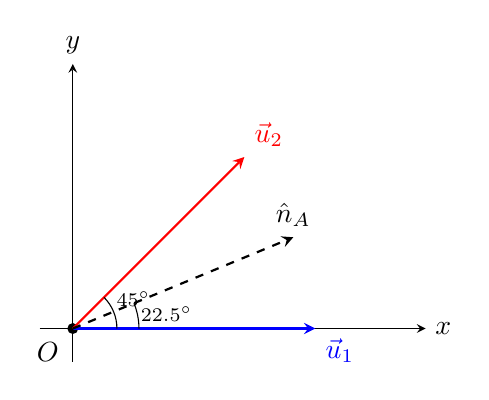
\begin{tikzpicture}[>=stealth, scale=1.4]
  \draw[->] (-0.3,0) -- (3.2,0) node[right] {$x$};
  \draw[->] (0,-0.3) -- (0,2.4) node[above] {$y$};
  \node[circle,fill,inner sep=1.4pt,label=below left:{$O$}] at (0,0) {};
  \draw[->,thick,blue] (0,0) -- (2.2,0) node[below right] {$\vec u_{1}$};
  \draw[->,thick,red] (0,0) -- (1.556,1.556) node[above right] {$\vec u_{2}$};
  \draw[->,thick,dashed] (0,0) -- (2.0,0.828) node[above] {$\hat n_{A}$};
  \draw (0.6,0) arc[start angle=0,end angle=22.5,radius=0.6];
  \node at (0.85,0.13) {\scriptsize $22.5^{\circ}$};
  \draw (0.4,0) arc[start angle=0,end angle=45,radius=0.4];
  \node at (0.55,0.27) {\scriptsize $45^{\circ}$};
\end{tikzpicture}
\end{center}

%==============================================================
\section*{Question 4 --- Constant force, 4-force, synchrotron}

\textbf{Problem.} (a) For constant $\vec F$ from rest find $\vec v(t)$ and show $|\vec v|\to c$. (b) Show $F^{\alpha}=(\gamma\vec F\cdot\vec v/c,\gamma\vec F)$ with $\vec F=m\gamma^{3}[\vec a+\vec v\times(\vec v\times\vec a)/c^{2}]$. (c) Compare radiative loss in linear vs circular accelerators. (d) Choose particle/machine to minimise loss.

\subsection*{(a)}
Integrate $\vec F=\de(\gamma m\vec v)/\de t$ from rest, with constant $\vec F$:
\[ \gamma m\vec v=\vec F t. \]
Take magnitude squared:
\[ \gamma^{2}m^{2}v^{2}=F^{2}t^{2}. \]
Substitute $\gamma^{2}v^{2}=v^{2}/(1-v^{2}/c^{2})$:
\[ \frac{m^{2}v^{2}}{1-v^{2}/c^{2}}=F^{2}t^{2}. \]
Clear the denominator:
\[ m^{2}v^{2}=F^{2}t^{2}-F^{2}t^{2}v^{2}/c^{2}. \]
Collect $v^{2}$ terms:
\[ v^{2}\big(m^{2}+F^{2}t^{2}/c^{2}\big)=F^{2}t^{2}. \]
Solve for $v^{2}$:
\[ v^{2}=\frac{F^{2}t^{2}}{m^{2}+F^{2}t^{2}/c^{2}}=\frac{(Ft/m)^{2}}{1+(Ft/(mc))^{2}}. \]
Take the positive root and align direction with $\vec F$:
\[ \boxed{\;\vec v(t)=\frac{\vec F t/m}{\sqrt{1+(Ft/(mc))^{2}}}.\;} \]
Take $t\to\infty$; numerator $\sim Ft/m$, denominator $\sim Ft/(mc)$:
\[ |\vec v(t)|\to\frac{Ft/m}{Ft/(mc)}=c. \]
Bounded limit:
\[ \boxed{\;\lim_{t\to\infty}|\vec v|=c.\;} \]

\subsection*{(b)}
Use $p^{0}=m\gamma c=E/c$ and $\de\tau=\de t/\gamma$ in the time component:
\[ F^{0}=\frac{\de p^{0}}{\de\tau}=\gamma\frac{\de p^{0}}{\de t}. \]
Substitute $p^{0}=E/c$:
\[ F^{0}=\frac{\gamma}{c}\frac{\de E}{\de t}. \]
Apply work-energy $\de E/\de t=\vec F\cdot\vec v$:
\[ F^{0}=\gamma\vec F\cdot\vec v/c. \]
Apply $\de\tau=\de t/\gamma$ to the spatial component, with $\vec F=\de\vec p/\de t$:
\[ F^{i}=\frac{\de p^{i}}{\de\tau}=\gamma\frac{\de p^{i}}{\de t}=\gamma F^{i}. \]
Combine into a 4-vector:
\[ \boxed{\;F^{\alpha}=(\gamma\vec F\cdot\vec v/c,\;\gamma\vec F).\;} \]
Expand $\vec F=\de(m\gamma\vec v)/\de t$:
\[ \vec F=m\frac{\de\gamma}{\de t}\vec v+m\gamma\vec a. \]
Substitute $\de\gamma/\de t=\gamma^{3}\vec v\cdot\vec a/c^{2}$:
\[ \vec F=\frac{m\gamma^{3}}{c^{2}}(\vec v\cdot\vec a)\vec v+m\gamma\vec a. \]
Apply BAC--CAB with $\vec A=\vec B=\vec v,\vec C=\vec a$:
\[ \vec v\times(\vec v\times\vec a)=(\vec v\cdot\vec a)\vec v-v^{2}\vec a. \]
Rearrange for $(\vec v\cdot\vec a)\vec v$:
\[ (\vec v\cdot\vec a)\vec v=\vec v\times(\vec v\times\vec a)+v^{2}\vec a. \]
Substitute into $\vec F$:
\[ \vec F=\frac{m\gamma^{3}}{c^{2}}\big[\vec v\times(\vec v\times\vec a)+v^{2}\vec a\big]+m\gamma\vec a. \]
Group the $\vec a$ terms:
\[ \vec F=m\gamma\!\Big(1+\frac{\gamma^{2}v^{2}}{c^{2}}\Big)\vec a+\frac{m\gamma^{3}}{c^{2}}\vec v\times(\vec v\times\vec a). \]
Apply $1+\gamma^{2}v^{2}/c^{2}=\gamma^{2}$:
\[ \vec F=m\gamma^{3}\vec a+\frac{m\gamma^{3}}{c^{2}}\vec v\times(\vec v\times\vec a). \]
Factor:
\[ \boxed{\;\vec F=m\gamma^{3}\!\left[\vec a+\frac{\vec v\times(\vec v\times\vec a)}{c^{2}}\right].\;} \]

\subsection*{(c)}
\textit{Linear case} ($\vec a\parallel\vec v$, so $\vec v\times\vec a=0$). From (b):
\[ F=m\gamma^{3}a. \]
Evaluate the Minkowski norm of $F^{\alpha}=(\gamma Fv/c,\gamma F\hat v)$ in $(-,+,+,+)$:
\[ F^{\alpha}F_{\alpha}=-\gamma^{2}F^{2}v^{2}/c^{2}+\gamma^{2}F^{2}=\gamma^{2}F^{2}(1-v^{2}/c^{2})=F^{2}. \]
Substitute $F^{2}=m^{2}\gamma^{6}a^{2}$:
\[ \left|\frac{\de p^{\alpha}}{\de\tau}\frac{\de p_{\alpha}}{\de\tau}\right|=m^{2}\gamma^{6}a^{2}. \]
Plug into the magnitude of Larmor's formula (taking $P>0$ as physical):
\[ P_{\mathrm{lin}}=\frac{q^{2}}{6\pi\epsilon_{0}m^{2}c^{3}}\,m^{2}\gamma^{6}a^{2}=\frac{q^{2}\gamma^{6}a^{2}}{6\pi\epsilon_{0}c^{3}}. \]
\textit{Circular case} ($\vec a\perp\vec v$). Apply BAC--CAB:
\[ \vec v\times(\vec v\times\vec a)=(\vec v\cdot\vec a)\vec v-v^{2}\vec a=-v^{2}\vec a. \]
Substitute into the (b) expression:
\[ \vec F=m\gamma^{3}\!\left[\vec a-\frac{v^{2}}{c^{2}}\vec a\right]. \]
Factor and use $\gamma^{2}(1-v^{2}/c^{2})=1$:
\[ \vec F=m\gamma^{3}(1-v^{2}/c^{2})\vec a=m\gamma\vec a. \]
With $\vec F\cdot\vec v=0$, the time component $F^{0}$ vanishes; the norm becomes:
\[ \left|\frac{\de p^{\alpha}}{\de\tau}\frac{\de p_{\alpha}}{\de\tau}\right|=\gamma^{2}F^{2}=\gamma^{2}(m\gamma a)^{2}=m^{2}\gamma^{4}a^{2}. \]
Plug into the magnitude of Larmor's formula:
\[ P_{\mathrm{circ}}=\frac{q^{2}}{6\pi\epsilon_{0}m^{2}c^{3}}\,m^{2}\gamma^{4}a^{2}=\frac{q^{2}\gamma^{4}a^{2}}{6\pi\epsilon_{0}c^{3}}. \]
Take the ratio at the same $\gamma$ and $a$ (as the question requests):
\[ \frac{P_{\mathrm{circ}}}{P_{\mathrm{lin}}}=\frac{\gamma^{4}a^{2}}{\gamma^{6}a^{2}}. \]
Simplify:
\[ \boxed{\;\frac{P_{\mathrm{circ}}}{P_{\mathrm{lin}}}=\frac{1}{\gamma^{2}},\qquad\text{equivalently }\frac{P_{\mathrm{lin}}}{P_{\mathrm{circ}}}=\gamma^{2}.\;} \]

\subsection*{(d)}
At fixed final energy $E$, write $\gamma=E/(mc^{2})$. For a ring of fixed radius $R$, the centripetal acceleration is:
\[ a=\frac{v^{2}}{R}\to\frac{c^{2}}{R}\quad(\gamma\gg 1). \]
Substitute into $P_{\mathrm{circ}}$:
\[ P_{\mathrm{circ}}=\frac{q^{2}\gamma^{4}a^{2}}{6\pi\epsilon_{0}c^{3}}\propto\frac{\gamma^{4}}{R^{2}}\propto\frac{E^{4}}{m^{4}R^{2}}. \]
In a linear machine, $\vec a\parallel\vec v$ and the radiated power for fixed accelerating force $F$ uses $F=m\gamma^{3}a$:
\[ P_{\mathrm{lin}}=\frac{q^{2}\gamma^{6}a^{2}}{6\pi\epsilon_{0}c^{3}}=\frac{q^{2}F^{2}}{6\pi\epsilon_{0}m^{2}c^{3}}. \]
At fixed $F$, $P_{\mathrm{lin}}\propto 1/m^{2}$ and is independent of $\gamma$, whereas $P_{\mathrm{circ}}$ grows as $\gamma^{4}\propto E^{4}/m^{4}$. Compare mass ratio $m_{\mu}/m_{e}\approx 207$:
\[ (m_{\mu}/m_{e})^{2}\approx 4.3\times 10^{4},\quad (m_{\mu}/m_{e})^{4}\approx 1.8\times 10^{9}. \]
Both factors favour the muon, and the linear geometry removes the $\gamma^{4}$ enhancement. Choose:
\[ \boxed{\;\text{muon in a linear accelerator}.\;} \]
Reasons: (i) linear geometry replaces $a=c^{2}/R$ with the (small) accelerating gradient, eliminating the $\gamma^{4}$ ring enhancement; (ii) the muon's larger rest mass suppresses Larmor by an extra $1/m^{2}$ at fixed accelerating force.

\end{document}
